\documentclass[a4paper]{article}

\usepackage[spanish]{babel}
\usepackage[utf8]{inputenc}
\usepackage{graphicx}
\usepackage{amsmath}
\usepackage[T1]{fontenc}
\usepackage{hyperref}
\usepackage{float}
\usepackage{longtable}


\title{Proyecto de investigación sobre detección de caras mediante OpenCV} 
\author{Alejandro Rodríguez Rodríguez \and Pablo Cano Navajas \and Salvador Caballero Macías}

\begin{document}

\maketitle

\newpage
\tableofcontents

\newpage
\section*{Resumen}

Este documento detalla las diferentes implementaciones que se han llevado a cabo durante la implementación de las mismas, asi como los resultados obtenidos y las conclusiones a las que se ha llegado. El proyecto se ha realizado empleando el repositorio\cite{1} que se detalla en el libro escogido\cite{2}.
De la documentacion escogida, se ha seleccionado el capítulo número 5, que trata sobre la detección de caras, tanto en imágenes como en captura en tiempo real, así como las implementaciones de mejoras de los algoritmos que se tratan en el libro para detectar un mayor número de caras o distintos objetos que cumplan unas restricciones que se impongan.

\section{Introducción}

El capítulo 5 del libro \textit{Learning OpenCV 4 Computer Vision with Python 3 Third Edition} \cite{2} se centra en la \textbf{detección y reconocimiento de caras}. Este capítulo introduce la funcionalidad de OpenCV para estas tareas, junto con los archivos de datos que definen tipos particulares de objetos rastreables. Se exploran los \textbf{clasificadores de cascada Haar}, que analizan el contraste entre regiones de imagen adyacentes para determinar si una imagen o subimagen coincide con un tipo conocido.

Un método clásico y ampliamente utilizado
para la detección de rostros es el uso de clasificadores en cascada de Haar,
implementados eficientemente en bibliotecas como OpenCV. Estos clasificadores
analizan el contraste entre regiones adyacentes de una imagen mediante un
conjunto de características similares a Haar organizadas en una estructura en
cascada para una rápida evaluación de posibles regiones de rostro. 
\begin{figure}[h!]
    \centering
    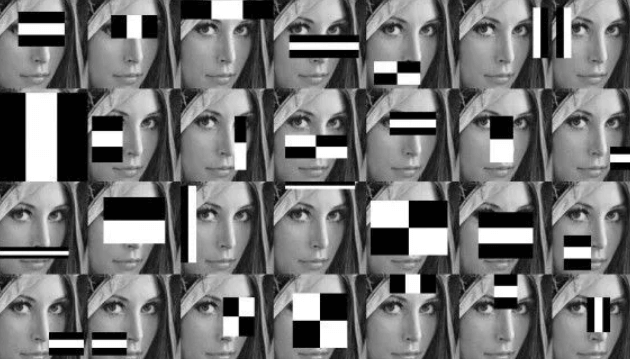
\includegraphics[width=0.6\textwidth]{../img/haar_cascade.png}
    \caption{Ejemplo de características Haar en una imagen.}
\end{figure}

Si bien esta
técnica ha demostrado ser efectiva en muchas situaciones, su rendimiento puede
verse afectado por diversos factores, como la escala, la orientación y las condiciones
de detección. En este trabajo, exploramos una mejora en la detección
de rostros utilizando los clasificadores en cascada de Haar mediante la optimizaci
ón de los parámetros del proceso de detección, buscando un equilibrio entre
la sensibilidad del detector y la reducción de falsos positivos.

\section{Planteamiento teórico}

El método de cascadas de Haar es una técnica de visión artificial ampliamente utilizada para la detección rápida y robusta de objetos, siendo la detección de rostros su aplicación más destacada y el contexto en el que fue introducido por primera vez. Esta técnica fue presentada en el influyente artículo ``Robust Real-Time Face Detection'' por Paul Viola y Michael Jones en 2001. El marco propuesto por Viola y Jones se basa en tres contribuciones principales que, combinadas, permiten un detector extremadamente rápido y fiable:

\begin{enumerate}
    \item \textbf{Características Haar-like:} En lugar de procesar directamente los píxeles brutos de una imagen, el sistema se basa en el uso de características simples denominadas ``Haar-like''. Estas características describen patrones de contraste entre regiones adyacentes de una sub-imagen. Funcionan calculando la diferencia entre la suma de los píxeles en áreas rectangulares blancas y negras dentro de una ventana de detección deslizante. Por ejemplo, pueden detectar bordes, vértices o líneas finas basándose en estos cambios de intensidad. El uso de características en lugar de píxeles directos ayuda a codificar conocimiento de dominio y permite que el sistema opere mucho más rápido. Además, para calcular estas características de forma extremadamente rápida, Viola y Jones introdujeron la representación de imagen conocida como ``Integral Image''.
    \item \textbf{Clasificador Simple y Eficiente con Selección de Características:} Se construye un clasificador potente combinando una colección de funciones de clasificación débiles. Para ello, se utiliza el algoritmo de aprendizaje AdaBoost. AdaBoost tiene la función dual de entrenar el clasificador y, crucialmente, seleccionar un pequeño número de características críticas de un conjunto muy grande de posibles características. Un clasificador débil se define como una función de clasificación que depende de una única característica Haar-like, junto con un umbral y una polaridad. Aunque ninguna característica individual por sí sola puede realizar la tarea de clasificación con un error bajo, AdaBoost permite seleccionar la característica rectangular que mejor separa los ejemplos positivos (por ejemplo, rostros) de los negativos en cada etapa del entrenamiento. La selección agresiva de características por parte de AdaBoost asegura que, aunque el conjunto inicial de características sea grande y complejo, el clasificador resultante sea computacionalmente eficiente ya que solo necesita evaluar un pequeño subconjunto de características durante la ejecución.
    \item \textbf{Estructura de Cascada:} La tercera contribución clave es el método para combinar clasificadores progresivamente más complejos en una estructura de cascada. Esta estructura es fundamental para lograr la detección en tiempo real. La idea central es que las sub-ventanas de la imagen que claramente no contienen el objeto buscado (por ejemplo, un rostro) pueden ser descartadas rápidamente en las etapas iniciales de la cascada, que consisten en clasificadores más simples y eficientes. Solo las regiones que superan la prueba de una etapa pasan a la siguiente etapa, que es ligeramente más compleja. Si una sub-ventana es rechazada en cualquier etapa, el procesamiento se detiene para esa región. Esta arquitectura de árbol de decisión degenerado reduce drásticamente la cantidad de cálculo necesario, enfocando el esfuerzo computacional solo en las regiones más prometedoras. Los experimentos demostraron que un clasificador en cascada podía ser significativamente más rápido que un clasificador monolítico con precisión comparable, debido a la capacidad de la primera etapa para descartar la mayoría de los no-objetos.
\end{enumerate}

En resumen, el planteamiento teórico de las cascadas de Haar para la detección de objetos se basa en el uso de características locales de contraste (Haar-like), la selección de las características más discriminatorias y el entrenamiento de clasificadores débiles mediante AdaBoost, y la organización de estos clasificadores en una cascada secuencial que permite un procesamiento extremadamente rápido al descartar eficientemente las regiones de fondo.

Implementaciones como la proporcionada por OpenCV incluyen datos de cascada pre-entrenados (en archivos XML) y métodos como \texttt{detectMultiScale}que manejan la aplicación de la cascada sobre una imagen. Para manejar la invariancia a la escala, la técnica típicamente reescala la imagen de entrada en múltiples tamaños, creando una pirámide de imágenes, mientras la ventana de detección mantiene un tamaño constante. Sin embargo, es importante notar que las cascadas de Haar, tal como se usan comúnmente, no son robustas a cambios significativos en la rotación o perspectiva del objeto.

A pesar de sus limitaciones con la rotación y perspectiva, la eficiencia y la capacidad de detección en tiempo real de las cascadas de Haar las han convertido en una técnica fundamental en visión artificial, a menudo utilizada en combinación con otras técnicas, como la información de profundidad para tareas de segmentación o intercambio de rostros.



\subsection{Conceptualizando las Cascadas de Haar}

El concepto de clasificación de objetos y el seguimiento de su ubicación buscan identificar qué constituye una parte reconocible de un objeto. Las imágenes fotográficas pueden contener muchos detalles, pero estos detalles pueden ser inestables debido a variaciones en la iluminación, el ángulo de visión, la distancia de visión, el movimiento de la cámara y el ruido digital. Afortunadamente, para la clasificación, no todas las diferencias en los detalles físicos son relevantes.

Las \textbf{características tipo Haar} son un tipo de característica que se aplica a menudo a la detección de rostros en tiempo real. 
\begin{figure}[h!]
    \centering
    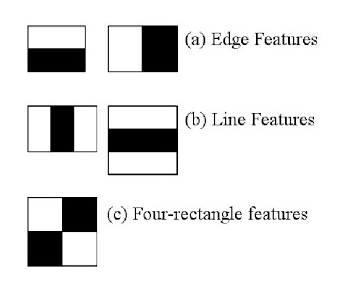
\includegraphics[width=0.6\textwidth]{../img/haar_feat.png}
    \caption{Tipos de características de Haar.}
\end{figure}

Estas características describen el patrón de contraste entre regiones de imagen adyacentes. Por ejemplo, los bordes, los vértices y las líneas delgadas generan un tipo de característica. Algunas características son distintivas en el sentido de que típicamente ocurren en una cierta clase de objeto (como una cara) pero no en otros objetos. Estas características distintivas se pueden organizar en una jerarquía, llamada \textbf{cascada}, en la que las capas superiores contienen características de mayor distinción, lo que permite que un clasificador rechace rápidamente los sujetos que carecen de estas características.

Las características pueden variar según la escala de la imagen y el tamaño del vecindario dentro del cual se evalúa el contraste, llamado \textbf{tamaño de ventana}. 

\begin{figure}[H]
    \centering
    \begin{minipage}[b]{0.32\textwidth}
        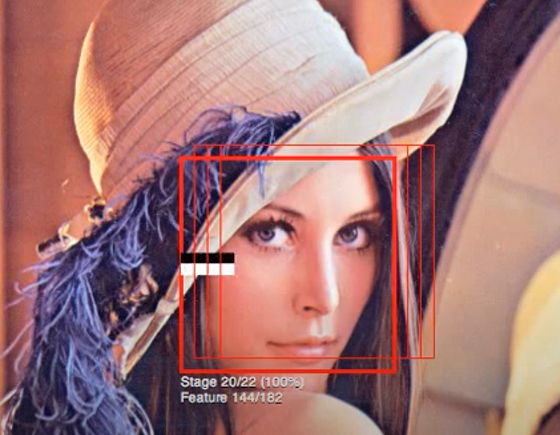
\includegraphics[width=\textwidth]{../img/hf1.png}
    \end{minipage}
    \hfill
    \begin{minipage}[b]{0.32\textwidth}
        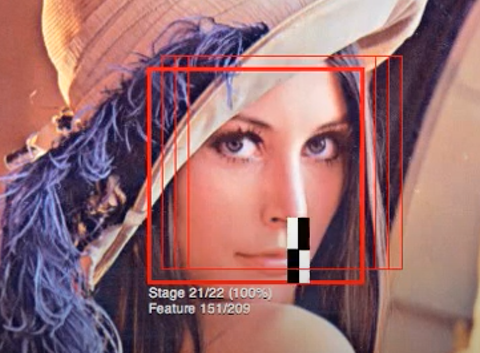
\includegraphics[width=\textwidth]{../img/hf2.png}
    \end{minipage}
    \hfill
    \begin{minipage}[b]{0.32\textwidth}
        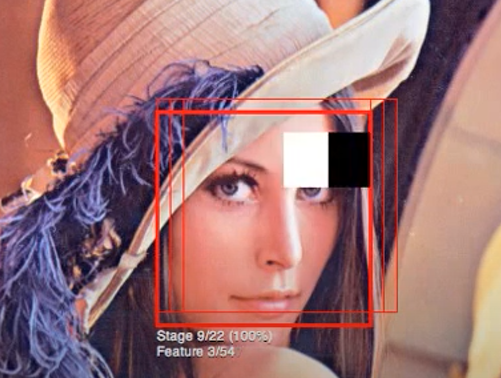
\includegraphics[width=\textwidth]{../img/hf3.png}
    \end{minipage}
    \caption{Ejemplo de características Haar en una imagen.}
\end{figure}

Para hacer que un clasificador de cascada Haar sea \textbf{invariante a la escala}, el tamaño de la ventana se mantiene constante pero las imágenes se reescalan varias veces; de esta manera, a algún nivel de reescalado, el tamaño de un objeto (como una cara) puede coincidir con el tamaño de la ventana. La imagen original y las imágenes reescaladas juntas se denominan \textbf{pirámide de imágenes}\cite{4}, y cada nivel sucesivo en esta pirámide es una imagen reescalada más pequeña. OpenCV proporciona un clasificador invariante a la escala que puede cargar una cascada Haar desde un archivo XML en un formato particular. Internamente, este clasificador convierte cualquier imagen dada en una pirámide de imágenes.

\subsection{Usando OpenCV para la Detección de Caras}

El código fuente de OpenCV 4, o una instalación preempaquetada, debería contener una subcarpeta llamada \texttt{data/haarcascades} . Esta carpeta contiene archivos XML que pueden ser cargados por una clase de OpenCV llamada \texttt{cv2.CascadeClassifier} . Una instancia de esta clase interpreta un archivo XML dado como una cascada Haar, que proporciona un modelo de detección para un tipo de objeto como una cara . \texttt{cv2.CascadeClassifier} puede detectar este tipo de objeto en cualquier imagen, ya sea una imagen fija de un archivo o una serie de fotogramas de un archivo de video o una cámara de video.

Para realizar la detección de caras, se puede crear un script básico que cargue un clasificador de cascada Haar para la detección de rostros y luego aplique este clasificador a una imagen. 

\begin{figure}[h!]
    \centering
    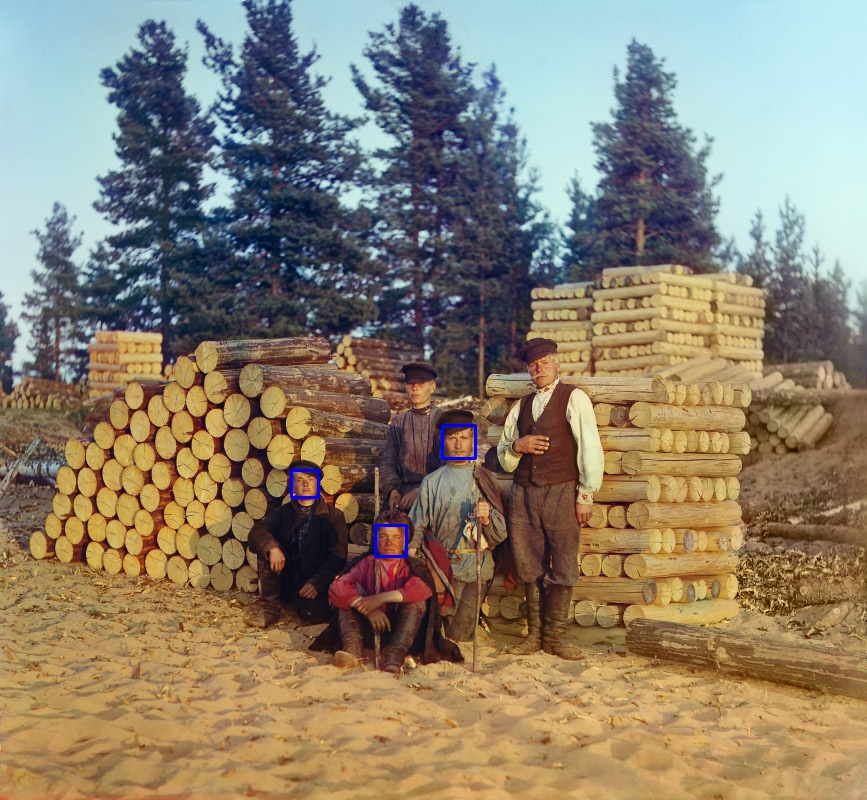
\includegraphics[width=0.6\textwidth]{../img/woodcutters_face_detection.jpg}
    \caption{Ejemplo de detección de caras.}
\end{figure}

\subsection{Mejorando el Clasificador de Cascadas de Haar}

La efectividad de un clasificador de cascada Haar puede verse afectada por los parámetros utilizados en la función \texttt{detectMultiScale}, como los atributos \texttt{scaleFactor} y \texttt{minNeighbors}.
En esta sección se explica cómo detectar caras tanto en imagenes como en una entrada de vídeo en tiempo real (e.g. una cámara de vídeo).
OpenCV proporciona herramientas avanzadas para el procesamiento de imágenes y la detección de objetos mediante el uso de clasificadores en cascada de Haar.\newline

\section{Implementación/Experimentación}

\subsection{Implementación de características de Cascadas de Haar}

En esta implementación vamos a experimentar en un archivo Notebook de Python con los filtros que utiliza el algoritmo de cascadas de Haar para obtener características propias de una cara. Este archivo lo podemos encontrar en la carpeta cascadas\_propias del repositorio del proyecto.

Para ello vamos a utilizar como referencia la siguiente imagen de una cara.

\begin{figure}[H]
    \centering
    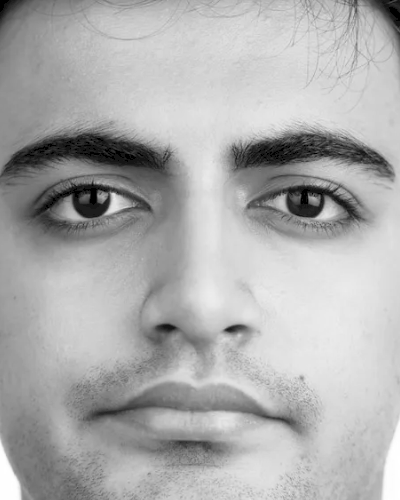
\includegraphics[width=0.40\textwidth]{../img/cara.png}
    \caption{Imagen de referencia del archivo cascadas.ipynb.}
\end{figure}

Los filtros o kernels que vamos a utilizar son los mismos que se muestran en el apartado 2.1 Conceptualizando las Cascadas de Haar.
Los cuales serán implementados de la siguiente manera; la parte blanca estará ocupada por -1's mientras que la parte negra estará ocupada por 1's.

\begin{figure}[H]
    \centering
    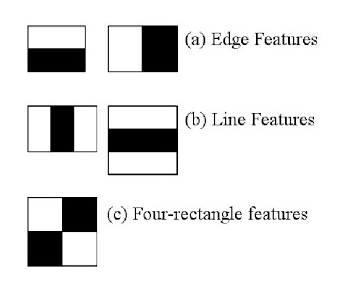
\includegraphics[width=0.6\textwidth]{../img/haar_feat.png}
    \caption{Kernels.}
\end{figure}

Lo primero que vamos a hacer será cargar la imagen original y redimensionarla a 300 x 300 píxeles.

Voy a crear los primeros dos kernels, los cuales se encargarán de mostrar \underline{características de bordes}.
Para ello voy a crear dos matrices de ceros y después modificaré el valor de las filas o columnas. La primera tendrá tamaño dos filas por tres columnas; la primera fila sera de -1's y la segunda de 1's.
La segunda matriz tendrá un tamaño de dos filas por cuatro columnas, donde las dos columnas de la izquieda serán de -1's y las dos columnas de la derecha tendrán valores de 1's.

\begin{figure}[H]
    \centering
    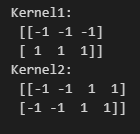
\includegraphics[width=0.3\textwidth]{../img/k1k2.png}
    \caption{Kernel1 y Kernel2.}
\end{figure}

Lo siguiente que voy a hacer será pasar estos filtros por la imagen de la cara original para poder visualizar que características resarta estos filtros.

\begin{figure}[H]
    \centering
    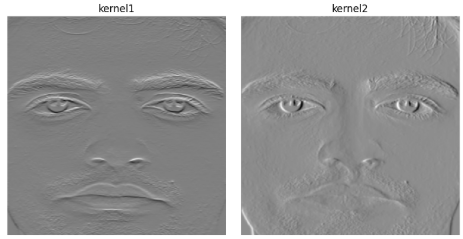
\includegraphics[width=0.80\textwidth]{../img/resultadok1k2.png}
    \caption{Resultado al aplicar kernel1 y kernel2 sobre la imagen original.}
    \label{f:f}
\end{figure}

Como se puede observar en la figura \ref{f:f} el kernel 1 nos sirve para destacar bordes horizontales.
Esto lo podemos ver en el borde entre los dos labios o en los bordes horizontales que podemos observar en los ojos, además se puede apreciar el borde en las cejas.

El kernel 2 destaca bordes verticales, esto lo podemos observar en los bordes que detecta este filtro sobre los ojos.
También se pueden apreciar algunas zonas verticales de la nariz.\\

Los siguientes dos kernels que voy a crear serán los encargados de destacar o resaltar \underline{características lineales}.
Para ello el kernel 3 tendrá una estructura de dos filas por tres columnas.
La columna central tendrá valores de 1's, mientra que las otras dos columnas tendrán valores de -1's.
El kernel 4 tendrá un tamaño de tres filas por tres columnas, la fila del medio tendrá valores de 1's, mientras que el resto de filas tendrá valor de -1's.

\begin{figure}[H]
    \centering
    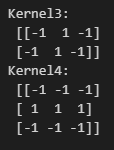
\includegraphics[width=0.30\textwidth]{../img/k3k4.png}
    \caption{Kernel3 y Kernel4.}
\end{figure}

\begin{figure}[H]
    \centering
    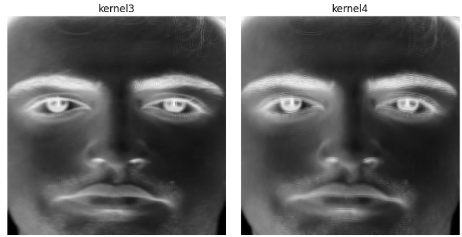
\includegraphics[width=0.80\textwidth]{../img/resultadok3k4.png}
    \caption{Resultado al aplicar kernel3 y kernel4 sobre la imagen original.}
    \label{fig:k3k4}
\end{figure}

Como se puede observar en la Figura \ref{fig:k3k4}, con estos dos filtros lo que vamos a destacar son características lineales.
Si observamos podemos ver que las cejas se muestran como dos lineas de color claro.
También se puede observar una linea oscura que recorre la nariz de arriba a abajo.
También podemos observar una linea algo más clara que corresponde con la boca.
Además se pueden ver los ojos como un circulo claro sobre un fondo más oscuro.

En estas dos imágenes se puede observar com mayor claridad lo que buscan las característica de haar.
La diferencia de contraste entre característica propias de un rostro.\\

Por último voy a implementar un kernel para \underline{características rectangulares}.
Este kernel tendrá tamaño cuatro filas por cuatro columnas, se dividirá en cuatro partes iguales como podemos ver a continuación.

\begin{figure}[H]
    \centering
    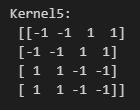
\includegraphics[width=0.30\textwidth]{../img/k5.png}
    \caption{Kernel5.}
\end{figure}

\begin{figure}[H]
    \centering
    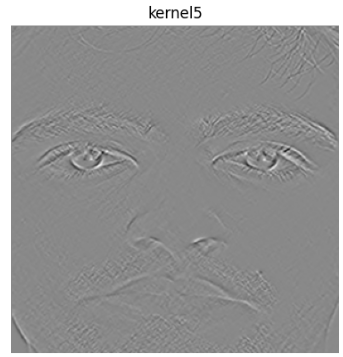
\includegraphics[width=0.50\textwidth]{../img/resultadok5.png}
    \caption{Resultado al aplicar el Kernel5.}
\end{figure}

Como se puede ver en la anterior imagen con este filtro se destacan característica rectangulares.
Como podemos ver alrededor de los ojos o incluso en las fosas nasales.\\



Con estas implementaciones nos podemos hacer una idea de las características que busca el algoritmo de Haar, para posteriomente aprender según las diferentes regiones de contraste que puede tener una cara.
Hay que tener en cuenta que cada cara es diferente, además depende de la luz, de si esa cara está girada hacia un lado o hacia otro; por ello el algoritmo necesita gran cantidad de imágenes de caras para poder tener en cuenta toda esta variabilidad.



\subsection{Implementación de Detección de Caras}

En el repositorio, dentro de la carpeta faceDetection, podemos encontrar una serie de archivos. El archivo \texttt{0\_stillImageFaceDetection} contiene el código para detectar imágenes estáticas con las explicaciones paso a paso del funcionamiento del algoritmo en inglés.Al final de dicho archivo se puede encontrar un apéndice con una explicación más extendida sobre ciertos parámetros o subrutinas de las funciones.

El método clave para realizar la detección de caras es \texttt{detectMultiScale}, que se aplica a una imagen en escala de grises. Los parámetros de \texttt{detectMultiScale} incluyen \texttt{scaleFactor} y \texttt{minNeighbors} (\textit{Ver anexo 2}). El argumento \texttt{scaleFactor}, que debe ser mayor que 1.0, determina la relación de reducción de escala de la imagen en cada iteración del proceso de detección de rostros. El argumento \texttt{minNeighbors} es el número mínimo de detecciones superpuestas que se requieren para conservar un resultado de detección.

También es posible realizar la detección de caras en un video utilizando una cascada Haar para rostros y otra para ojos. El proceso implica capturar fotogramas de una cámara, convertirlos a escala de grises y luego aplicar el detector de rostros. Para cada rostro detectado, se puede definir una región de interés (ROI) y aplicar un detector de ojos dentro de esa ROI.

El \texttt{scaleFactor} influye en la robustez a diferentes tamaños de rostro, mientras que \texttt{minNeighbors} ayuda a reducir los falsos positivos al requerir múltiples detecciones superpuestas. Ajustar estos parámetros mediante experimentación puede mejorar el rendimiento del detector en diferentes condiciones de iluminación y para diferentes sujetos. Además, el uso de múltiples clasificadores en cascada, como uno para la detección frontal de rostros y otro para la detección de ojos dentro de la región facial detectada, puede aumentar la precisión de la detección de características específicas.

\begin{figure}[h!]
    \centering
    \begin{minipage}[b]{0.48\textwidth}
        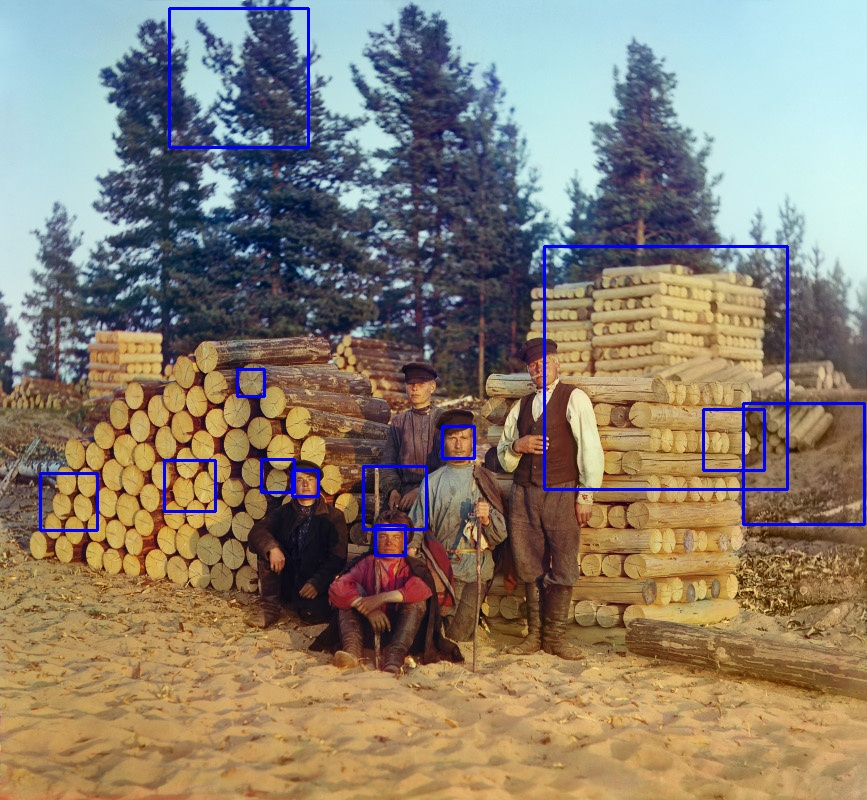
\includegraphics[width=\textwidth]{../img/woodcutters_face_detection103.jpg}
        \caption{Ejemplo de detección con un índice de 1.03}
    \end{minipage}
    \hfill
    \begin{minipage}[b]{0.48\textwidth}
        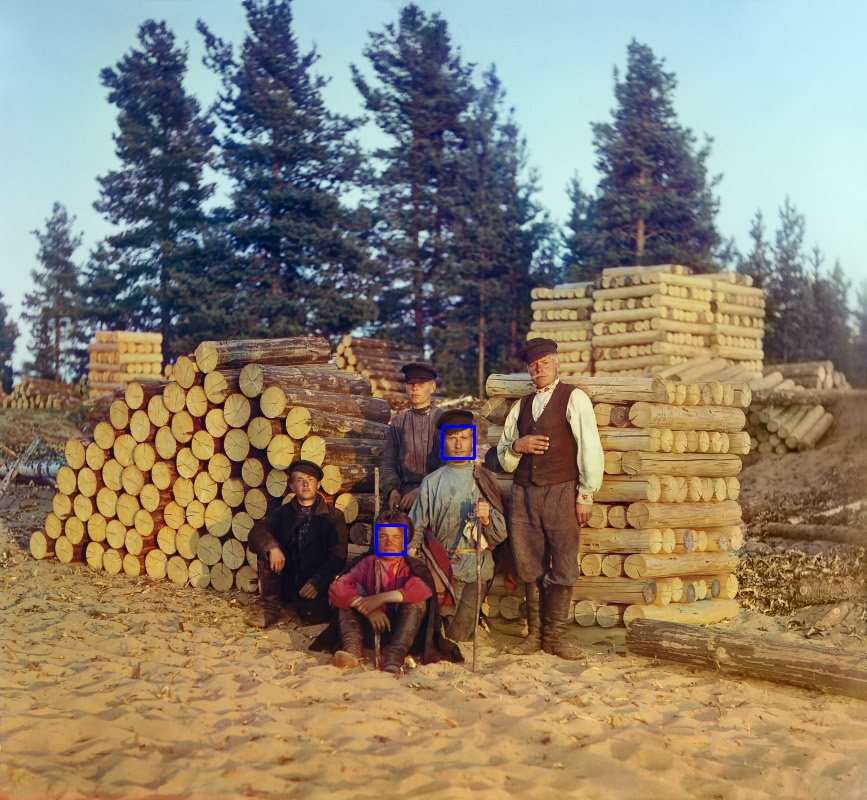
\includegraphics[width=\textwidth]{../img/woodcutters_face_detection11.jpg}
        \caption{Ejemplo de detección con un índice de 1.1}
    \end{minipage}
\end{figure}

Este factor hace que se desescale la imagen iterativamente, es decir, comienza con un tamaño de ventana dado, itera sobre la imagen detectando las caracteristicas de haar y se acumulan las detecciones posibles que se hayan podido dar en esa iteracion. En la siguiente, se desescala la imagen, si el factor de escala es 1.1, se desescala un 10\% y se vuelve a iterar las caracteristicas de haar. Es importante saber que al desescalar la imagen estaremos detectando características de haar más grandes. El factor toma valores a partir de 1. Cuanto más cercano a 1 esté más tardará el algoritmo en detectar las caras pero más fiable.

Como se puede apreciar en la primera figura, al tener un valor bajo detectará muchos recuadros, dando así falsos positivos. Si aumentamos excesivamente el valor, como se muestra en la figura 7, el algoritmo no detectará correctamente las caras.

\begin{figure}[h!]
    \centering
    \begin{minipage}[b]{0.48\textwidth}
        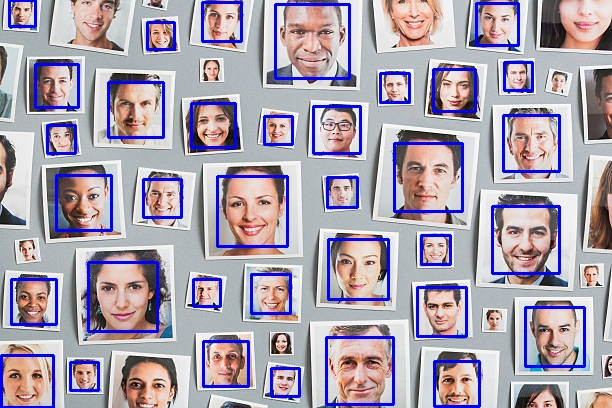
\includegraphics[width=\textwidth]{../img/multImages_face_detection103.jpg}
        \caption{Ejemplo de detección con un índice de 1.03}
    \end{minipage}
    \hfill
    \begin{minipage}[b]{0.48\textwidth}
        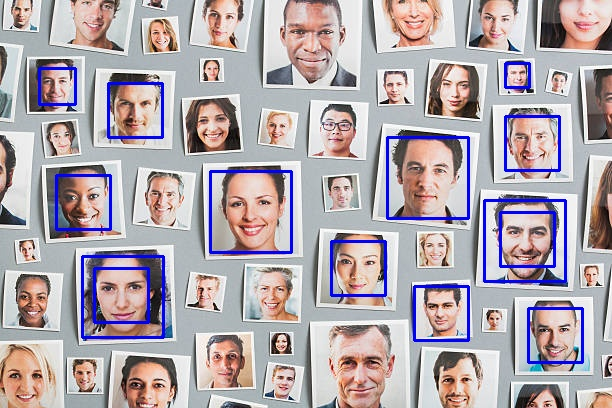
\includegraphics[width=\textwidth]{../img/multImages_face_detection15.jpg}
        \caption{Ejemplo de detección con un índice de 1.5}
    \end{minipage}
\end{figure}

Lo mismo ocurre en el caso de la figura 8, donde el índice de 1.03 detecta más caras que el índice de 1.5. En este caso, el índice de 1.03 permite una mayor variación en la escala de las imágenes, lo que resulta en más detecciones, mientras que un índice de 1.5 reduce la cantidad de detecciones al aumentar el tamaño de la ventana de búsqueda.

Para utilizar un clasificador de cascada Haar en OpenCV para la detección de caras, el primer paso es cargar el archivo XML de la cascada utilizando la función \texttt{cv2.CascadeClassifier()} :

La detección de caras se realiza utilizando archivos XML que contienen los datos preentrenados para identificar características faciales específicas. Estos clasificadores se cargan mediante la función \texttt{cv2.CascadeClassifier}, que permite aplicar los modelos a imágenes o fotogramas de vídeo.
El proceso incluye los siguientes pasos:

\begin{itemize}
    \item Carga de la imagen mediante \texttt{cv2.imread}.
    \item Conversión de la imagen a escala de grises para optimizar el rendimiento del clasificador.
    \item Uso del clasificador \texttt{haarcascade\_frontalface\_default.xml} para detectar caras.
\end{itemize}

El script \texttt{1\_cameraFaceDetection.ipynb} permite realizar la detección de caras en tiempo real utilizando la cámara del dispositivo. A continuación, se describen los pasos principales que realiza el script:
Este script es útil para aplicaciones en las que se requiere detección de rostros en tiempo real, como sistemas de seguridad o análisis de video en vivo.

\begin{itemize}
    \item Captura de vídeo en tiempo real mediante \texttt{cv2.VideoCapture}.
    \item Aplicación del clasificador en cascada a cada fotograma del vídeo.
    \item Detección de características adicionales, como ojos, utilizando el archivo \texttt{haarcascade\_eye.xml}.
\end{itemize}

El script \texttt{1\_cameraFaceDetection.ipynb} implementa la detección de caras en tiempo real utilizando la cámara del dispositivo. Este proceso incluye:

\begin{itemize}
    \item \textbf{Inicialización de la cámara}: Se utiliza la función \texttt{cv2.VideoCapture(0)} para acceder a la cámara del dispositivo. El argumento \texttt{0} indica que se usará la cámara predeterminada.
    \item \textbf{Conversión a escala de grises}: Cada fotograma capturado se convierte a escala de grises mediante la función \texttt{cv2.cvtColor}, lo que mejora el rendimiento del clasificador.
    \item \textbf{Detección de caras}: Se aplica el clasificador Haar cargado desde el archivo \texttt{haarcascade\_frontalface\_default.xml} para detectar rostros en cada fotograma.
    \item \textbf{Dibujar rectángulos}: Por cada rostro detectado, se dibuja un rectángulo alrededor de la región detectada utilizando la función \texttt{cv2.rectangle}.
    \item \textbf{Visualización en tiempo real}: Los fotogramas procesados se muestran en una ventana utilizando \texttt{cv2.imshow}, permitiendo observar las detecciones en tiempo real.
    \item \textbf{Finalización del script}: El bucle de captura se detiene al presionar una tecla específica (por ejemplo, \texttt{q}), y se liberan los recursos de la cámara con \texttt{cap.release()}.
\end{itemize}


\subsection{Impementación de proyecto cameo (Intercambio de caras)}

En este apartado voy a implementar el proyecto cameo, el cual consistirá en la detección de caras para su posterior intercambio.
Es decir, si se detectan dos caras con la cámara se dibujará un rectangulo alrededor de ellas y se intercambiarán una con la otra; si se detectan más de dos caras se realizará una cola circular para intercambiar todas las caras.

Las funciones que nos importan están debidamente comentadas en el repositorio del proyecto, en este documento voy a dar una explicación general.\\

Este proyecto está implementado en la carpeta cameo\_pid del repositorio del proyecto.
Como archivo principal del proyecto tenemos el fichero cameo.py el cual será el único que debamos ejecutar para que se abra la ventana de visualización de la cámara para poder ver como al detectar dos o más caras se produce el intercambio.

Este archivo está dividido en varias funciones; estas funciones se encargaran de abrir una ventana de visualización usando la cámara predeterminada del sistema.
Se van capturando fotograma a fotograma y se pasan al fichero trackers.py que será el encargado de detectar si en la imagen aparece algún rostro.
En este archivo también tenemos un manejador de eventos, el cual se encarga de detectar si se pulsa alguna de las teclas que a nosotros nos importa; al pulsa la barra de espacio se guarda el fotograma actual, si se pulsa el tabulador se activa una pequeña grabación de la ventana de visualización, si se pulsa la letra 'x' se activa o desactiva el rectángulo alrededor de la cara y de los ojos y por último para cerrar la ventana de visualización se debe pulsar la tecla de 'scape'.

El fichero trackers.py que ya he nombrado, se encarga de detectar si en el fotograma que se pasa contiene algún rostro, para ello hace uso de los clasificadores de Cascadas de Haar preentrenados.
Una vez que detecta un rostro se queda con la subimagen que contiene dicho rostro para comprobar que de verdad es un rostro, para ello en esta subimagen se busca en la parte en la que se supone que debe estar el ojo izquierdo si de verdad está y lo mismo para el ojo derecho.

Estos ficheros nombrados anteriomente hacen uso del fichero rects.py el cual se encarga de dibujar un rectángulo sobre cada una de las caras detectadas. Si solo detecta una cara no hará nada, si detectan dos caras se intercambian los rectángulos y si hay más de dos caras se intercambian de forma circular según hayan sido detectadas.




\section{Manual de usuario}

Para el correcto funcionamiento de los scripts, es necessario la instalación de los siguientes paquetes:

\begin{itemize}
    \item \textbf{Windows 7, MacOS 10.7 o superior}.
    \item \textbf{Python 3.8 o superior}. Para instalar Python, se recomienda instalar la versión más reciente accediendo a la página web \href{https://www.python.org/downloads/}{Python.org}. Haremos click en el botón de descarga y se descargará automáticamente el ejecutable. Si fuese necesario otra versión de python, en la misma págna se puede descargar la versión que se necesite.\\
    Si se tiene instalado un sistema operativo distinto a windows, se puede acceder al enlace de \href{https://www.python.org/downloads/macos/}{versiones macOS} y descargar la que sea necesaria siempre que cumpla con los requisitos de instalación.
    \item \textbf{OpenCV 4.0 o superior}. Para instalar la version 4.0 o superior de OpenCV, se recomienda usar el gestor de paquetes \texttt{pip}. Para ello, se abre una terminal y se ejecuta el comando \texttt{pip install opencv-python}. Si la máquina opera con macOS, se recomienda usar \texttt{brew}, escribiendo el comando \texttt{brew install opencv}.
    \item \textbf{NumPy 1.16 o superior}. Para instalarlo, en una ventana de comandos escribiremos \texttt{pip install numpy} (para un entorno Windows) o \texttt{brew install numpy} (para un entorno macOS).
    \item \textbf{Scipy 1.1 o superior}. Para instalarlo, en una ventana de comandos escribiremos \texttt{pip install scipy} (para un entorno Windows) o \texttt{brew install scipy} (para un entorno macOS).

\end{itemize}

\subsection{Instalación de Latex en Visual Studio Code}

Para poder instalar Latex en visual studio code, es necesario instalar los siquientes paquetes:

\begin{itemize}
    \item \textbf{Visual Studio Code}. Para instalarlo, se puede acceder a la página web \href{https://code.visualstudio.com/}{Visual Studio Code} y descargar el instalador correspondiente al sistema operativo que se esté utilizando.
\end{itemize}

\begin{figure}[h!]
    \centering
    
\includegraphics[width=0.6\textwidth]{../img/vsc.png}
    \caption{Página de descarga de Visual Studio Code.}
\end{figure}

\begin{itemize}
    \item \textbf{Latex Workshop}. Para instalarlo, abrimos Visual Studio Code y se accederemos a la pestaña de extensiones (icono de cuatro cuadrados en la barra lateral izquierda). En el campo de búsqueda, escribimos \texttt{latex workshop} y seleccionaremos la opción correspondiente (figura 9). Hacemos click en el botón de instalar.
\end{itemize}

\begin{figure}[h!]
    \centering
    
\includegraphics[width=0.6\textwidth]{../img/extensions.png}
    \caption{Instalación de Latex Workshop.}
\end{figure}

\begin{itemize}
    \item \textbf{MikTeX}. Para instalarlo, se puede acceder a la página web \href{https://miktex.org/download}{MikTeX} y descargar el instalador correspondiente al sistema operativo que se esté utilizando. Una vez descargado, ejecutamos el instalador y seguimos las instrucciones para completar la instalación.
\end{itemize}
    
\begin{figure}[h!]
    \centering
    
\includegraphics[width=0.6\textwidth]{../img/miktex.png}
    \caption{Página de descarga de MikTeX.}
\end{figure}
    

Al final de la instalación se nos preguntará si queremos chequear si hay actualizaciones. Se recomienda chequear la opción para mantenerlo actualizado y evitar errores futuros.
Para crear un nuevo fichero latex, crearemos el fichero con la extensión \texttt{.tex} y lo guardaremos en la carpeta donde se encuentre el proyecto. Para compilar el fichero, haremos click en el icono de \texttt{>} que aparece en el menú de arriba a la derecha en color verde y seleccionaremos la opción de compilar el documento. Esto generará un archivo PDF con el mismo nombre que el archivo \texttt{.tex}.

Es posible que en el proceso de compilación del archivo aparezcan ventanas emergentes pidiendo instalar una serie de paquetes necesarios, instalaremos todos y cuando termine la instalación de todos estos paquetes, se abrirá el archivo compilado en formato PDF. Si no se abre automáticamente, podemos abrirlo manualmente haciendo click en el icono de \texttt{View Latex PDF File} que aparece 2 iconos a la derecha (icono con la lupa) de la opción de compilación (>) como se muestra en la figura 11. Si no aparece, podemos abrirlo manualmente desde la carpeta donde se guardó el archivo \textit{.tex} haciendo click derecho y selecionando la opción \textit{Open to the Side}.

\begin{figure}[h!]
    \centering
    
\includegraphics[width=0.6\textwidth]{../img/menu.png}
    \caption{Opciones del menú de la barra superior.}
\end{figure}

\section{Conclusiones}

Hemos aprendido a implementar un algoritmo de detección de caras utilizando el algoritmo de cascadas de Haar. Este algoritmo es capaz de detectar rostros en imágenes y vídeos en tiempo real, lo que lo convierte en una herramienta valiosa para aplicaciones de visión por computadora.
Además, hemos explorado la implementación de un proyecto de intercambio de caras utilizando la detección de rostros. Este proyecto demuestra la versatilidad y el potencial del algoritmo de cascadas de Haar en aplicaciones creativas y entretenidas.
Hemos aprendido a utilizar OpenCV para la detección de rostros y a ajustar los parámetros del algoritmo para mejorar su rendimiento. También hemos explorado la importancia de la preprocesamiento de imágenes y la conversión a escala de grises para optimizar el rendimiento del clasificador.
\section{Autoevaluación de cada miembro}

\subsection{Autoevaluación de Alejandro}

Creo que en general he realizado un buen trabajo en la implementación del algoritmo de detección de caras utilizando el algoritmo de cascadas de Haar. He aprendido a utilizar OpenCV para la detección de rostros y a ajustar los parámetros del algoritmo para mejorar su rendimiento.
En relación a la organización del trabajo, quizás no he sido lo suficientemente organizado en la gestión del tiempo y la planificación de las tareas. En el futuro, me gustaría mejorar en este aspecto y asegurarme de que todas las tareas se realicen de manera oportuna y eficiente.
He dedicado un tiempo considerable a la investigación y la experimentación con el algoritmo de cascadas de Haar, lo que me ha permitido comprender mejor su funcionamiento y sus aplicaciones. Sin embargo, creo que podría haber dedicado más tiempo a la documentación del proyecto y a la creación de un manual de usuario más detallado.

\subsection{Autoevaluación de Pablo}

A lo largo de este proyecto, me he dedicado al estudio e implementación del algoritmo de detección de caras utilizando cascadas de Haar. Considero que la implementación del algoritmo ha sido, en general, satisfactoria. He adquirido un conocimiento práctico en el uso de la biblioteca OpenCV para la detección de rostros y he logrado experimentar con diversos parámetros del algoritmo, lo que me ha permitido optimizar su rendimiento en diferentes escenarios.

En cuanto a la organización del trabajo, reconozco que la gestión del tiempo y la planificación de las tareas podrían haber sido más eficientes. 

La investigación y experimentación con el algoritmo de cascadas de Haar han consumido una parte considerable de mi tiempo, lo cual me ha brindado una comprensión profunda de su funcionamiento interno y sus diversas aplicaciones. 
\subsection{Autoevaluación de Salvador}

Aunque no he llegado al tiempo óptimo de 70 horas creo que he realizado buen trabajo; ya que me he quedado cerca de las 67 horas.
Creo que los objetivos propuestos para mi trabajo han sido resueltos satisfactoriamente, he completado el proyecto para intercambio de caras y he experimentado con los filtros que usa el algoritmo de cascadas de Haar.
Además he seguido aprendiendo OpenCV, el cual comenzamos a usarlo en las clases de teoría.
También he aprendido como funciona la detección de objetos usando Cascadas de Haar.

\section{Tabla de tiempos}

\subsection{Tabla de tiempos de Alejandro}

\newpage

\begin{center}
\begin{longtable}{|c|c|c|p{8cm}|}
\hline
\textbf{Fecha} & \textbf{Tiempos (min)} & \textbf{Miembro} & \textbf{Actividad Realizada} \\
\hline
\endfirsthead
\hline
\textbf{Fecha} & \textbf{Tiempos (min)} & \textbf{Miembro} & \textbf{Actividad Realizada} \\
\hline
\endhead
16-feb & 110 & Alejandro & Sesión de seguimiento \\
03-mar & 30  & Alejandro & Lectura de documentación \\
03-mar & 90  & Alejandro & Implementación de algoritmos base \\
04-mar & 90  & Alejandro & Implementación de algoritmos base \\
09-mar & 90  & Alejandro & Lectura de documentación \\
12-mar & 110 & Alejandro & Sesión de seguimiento \\
22-mar & 120 & Alejandro & Implementación de algoritmos base \\
25-mar & 110 & Alejandro & Implementación de mejoras de algoritmos \\
26-mar & 110 & Alejandro & Sesión de seguimiento \\
30-mar & 150 & Alejandro & Implementación de mejoras de algoritmos \\
01-abr & 110 & Alejandro & Documentación \\
02-abr & 110 & Alejandro & Documentación \\
05-abr & 150 & Alejandro & Documentación \\
07-abr & 90  & Alejandro & Implementación de algoritmos base \\
08-abr & 110 & Alejandro & Documentación \\
09-abr & 110 & Alejandro & Sesión de seguimiento \\
14-abr & 120 & Alejandro & Documentación \\
16-abr & 60  & Alejandro & Documentación \\
16-abr & 120 & Alejandro & Investigación sobre posible mejora de detección de caras \\
17-abr & 150 & Alejandro & Investigación \\
22-abr & 90  & Alejandro & Documentación \\
22-abr & 60  & Alejandro & Documentación \\
23-abr & 60  & Alejandro & Documentación \\
29-abr & 60  & Alejandro & Documentación \\
30-abr & 110 & Alejandro & Sesión de seguimiento \\
30-abr & 90  & Alejandro & Documentación \\
30-abr & 90  & Alejandro & Experimentación \\
03-may & 120 & Alejandro & Documentación \\
04-may & 120 & Alejandro & Experimentación detección de caras en imágenes \\
05-may & 120 & Alejandro & Experimentación detección de caras en imágenes \\
05-may & 60  & Alejandro & Escritura presentación PowerPoint \\
06-may & 120 & Alejandro & Experimentación detección de caras en imágenes \\
07-may & 60  & Alejandro & Documentación \\
07-may & 60  & Alejandro & Experimentación \\
07-may & 60  & Alejandro & Escritura presentación PowerPoint \\
08-may & 60  & Alejandro & Documentación \\
08-may & 120 & Alejandro & Comprobación de la redacción de la documentación \\
08-may & 60  & Alejandro & Escritura presentación PowerPoint \\
09-may & 120 & Alejandro & Escritura presentación PowerPoint \\
10-may & 60  & Alejandro & Preparación presentación \\
10-may & 90  & Alejandro & Revisión final del proyecto \\
11-may & 120 & Alejandro & Preparación presentación \\
12-may & 120 & Alejandro & Preparación presentación \\
13-may & 120 & Alejandro & Preparación presentación \\
\hline
\end{longtable}
\end{center}

\subsection{Tabla de tiempos de Pablo}

\begin{table}[H]
    \centering
    \begin{tabular}{|c|p{10cm}|c|}
    \hline
    \textbf{Fecha} & \textbf{Tarea} & \textbf{Tiempo} \\
    \hline
    12/02/2025 & Elección tema y lectura documentación & 2 horas \\
    26/02/2025 & Sesión de Seguimiento & 2 horas \\
    26/02/2025 & Implementación cascadas de Haar & 2 horas \\
    09/03/2025 & Lectura documentación e implementación cascadas Haar & 1 hora 30 min \\
    15/03/2025 & Pruebas iniciales & 2 horas \\
    22/03/2025 & Ajustes de parámetros & 1 hora 30 min \\
    29/03/2025 & Documentación & 2 horas \\
    02/04/2025 & Implementación de detección en vídeo & 2 horas \\
    04/04/2025 & Depuración & 1 hora 30 min \\
    06/04/2025 & Documentación & 2 horas \\
    08/04/2025 & Documentación & 2 horas \\
    17/04/2025 & Documentación LaTeX & 2 horas \\
    18/04/2025 & Documentación LaTeX & 3 horas \\
    19/04/2025 & Escritura de la sección teórica sobre cascadas de Haar en LaTeX & 2 horas \\
    21/04/2025 & Búsqueda y selección de referencias y citas para la documentación & 2 horas \\
    23/04/2025 & Inserción de imágenes, esquemas & 2 horas \\
    24/04/2025 & Revisión de formato, bibliografía y consistencia en LaTeX & 2 horas \\
    25/04/2025 & Revisión técnica del apartado Haar & 2 horas \\
    26/04/2025 & Ajuste de figuras, tablas & 1 hora 30 min \\
    01/05/2025 & Documentación Artículo Cascadas Haar & 4 horas \\
    02/05/2025 & Desgranar funcionamiento Cascadas Haar & 4 horas \\
    03/05/2025 & Redactar funcionamiento Cascadas Haar & 4 horas \\
    04/05/2025 & Redactar funcionamiento Cascadas Haar & 4 horas \\
    05/05/2025 & Plantear las Cascadas Haar para la exposición & 4 horas \\
    06/05/2025 & Redactar explicación simplificada & 4 horas \\
    07/05/2025 & Preparar la Presentación & 4 horas \\
    08/05/2025 & Preparar la Presentación & 2 horas \\
    09/05/2025 & Preparar la Presentación & 2 horas \\
    10/05/2025 & Preparar la Presentación & 2 horas \\
    \textbf{Tiempo total} & & 71 horas \\
    \hline
    \end{tabular}
    \caption{Registro de tareas y tiempos del proyecto (Pablo)}
    \end{table}
    

\subsection{Tabla de tiempos de Salvador}

\begin{table}[H]
\centering
\begin{tabular}{|c|p{10cm}|c|}
\hline
\textbf{Fecha} & \textbf{Tarea} & \textbf{Tiempo} \\
\hline
12/02/2025 & Elección tema y recursos & 1 hora 30 min \\
24/02/2025 & Lectura documentación de referencia & 45 min \\
26/02/2025 & Lectura documentación de referencia e implementación de algoritmo básico & 1.30 hora \\
09/03/2025 & Lectura documentación de referencia e implementación de algoritmo básico. & 1.30 hora \\
24/03/2025 & Implementación en repositorio del algoritmo de intercambio de caras & 2 horas \\
25/03/2025 & Implementación en repositorio del algoritmo de intercambio de caras & 2 horas \\
28/03/2025 & Implementación en repositorio del algoritmo de intercambio de caras & 3 horas \\
31/03/2025 & Modificación algoritmo intercambio de caras & 2 horas \\
01/04/2025 & Modificación algoritmo intercambio de caras & 2 horas \\
02/04/2025 & Modificación algoritmo intercambio de caras e investigación funcionamiento cascadas de Haar & 2 horas \\
04/04/2025 & Investigación funcionamiento cascadas de Haar & 3 horas \\
06/04/2025 & Investigación e implementación cascadas de Haar paso a paso & 3 horas \\
07/04/2025 & Implementación cascadas de Haar paso a paso & 1 hora \\
08/04/2025 & Comienzo con la escritura de la documentación & 2 horas \\
22/04/2025 & Lectura de la documentación “Robust Real-Time Face Detection Viola and Jones” durante la clase & 2 horas \\
24/04/2025 & Implementación filtro cascadas de haar(documento cascadas de haar propias). Construcción de los kernels. & 2 horas \\
29/04/2025 & Implementación filtros cascadas de haar (documento cascadas de haar propias )  y añado comentarios a este mismo documento. Creación de la presentación del trabajo grupal. Creación de documento del seguimiento 4 & 5 horas \\
02/05/2025 & Experimentacion/implementacion filtros cascadas de haar(cascadas de har propias) & 1 hora \\
04/05/2025 & Experimentacion/implementacion filtros cascadas de haar(cascadas de har propias) & 2 horas \\
05/05/2025 & Experimentacion/implementacion filtros cascadas de haar(cascadas de har propias) & 3 horas \\
07/05/2025 & Añadir comentarios a los archivo cameo.py, facetracker.py y rect.py. Experimentacion/implementacion filtros cascadas de haar(cascadas de har propias) y añadir comentarios a cascadas propias & 4 horas \\
08/05/2025 & Experimentacion/implementacion filtros cascadas de haar(cascadas de har propias) y añadir comentarios. Instalacion de latex para poder escribir en visual studio & 5 horas 30 min \\
09/05/2025 & Escritura de la documentacion en latex & 5 horas \\
10/05/2025 & Escritura de la documentacion en latex & 3 horas \\
11/05/2025 & Comenzar presentacion y repasar archivo latex & 3 horas \\
12/05/2025 & Respaso archivo latex, escribir archivo readme, terminar y repasar presentación & 4 horas \\
\textbf{Tiempo total} & & 66 horas 45 min\\
\hline
\end{tabular}
\end{table}

\newpage
\begin{thebibliography}{99}
\bibitem{1} \textit{Repositorio del proyecto}, disponible en \href{https://github.com/PacktPublishing/Learning-OpenCV-4-Computer-Vision-with-Python-Third-Edition}{GitHub}
\bibitem{2} Joseph Howse, Joe Minichino, \textit{Learning OpenCV 4 Computer Vision with Python 3}", Third edition, Packt Publishing, pp. 1-372, 2020
\bibitem{3} \textit{Vídeo de detección de características Haar}, disponible en \href{https://youtu.be/hPCTwxF0qf4}{YouTube}
\bibitem{4} \textit{Pyramid (image processing)}, disponible en \href{https://en.wikipedia.org/wiki/Pyramid_(image_processing)}{Wikipedia}
\bibitem{5} \textit{OpenCV Cascade Classifier}, disponible en \href{https://docs.opencv.org/3.4/db/d28/tutorial_cascade_classifier.html}{docs.opencv.org}
\bibitem{6} \textit{Robust Real-Time Face Detection. Viola and Jones}, disponible \href{https://www.face-rec.org/algorithms/Boosting-Ensemble/16981346.pdf}{aquí}
\bibitem{7} \textit{Viola, Paul, y Michael J. Jones. «Robust Real-Time Face Detection». International Journal of Computer Vision 57, n.º 2 (1 de mayo de 2004): 137-54. https://doi.org/10.1023/B:VISI.0000013087.49260.fb.
}
\end{thebibliography}


\newpage
\section*{Anexos}
\textbf{|1|} Como se aprecia en la imagen, el cuadrado en rojo indica la posicion de la cara detectada, dentro de este cuadrado se encuentran los elementos de caracteristicas haar, que van iterando sobre la imagen y detectando las facciones de la imagen (tanto ojos, nariz, boca, etc.).

\end{document}